% Cours pour débutant : tout le projet A1 (filtrage collaboratif), groupe 40 « La piscine ».
% Compilation (depuis docs/cours/) : pdflatex cours_methodes.tex (deux fois, pour la table des matières).
% Les figures sont lues dans ../../figures/ (produites par experiments/*.py) et dans ce dossier.
\documentclass[11pt,a4paper]{article}

\usepackage[T1]{fontenc}
\usepackage[utf8]{inputenc}
\usepackage[french]{babel}
\usepackage{lmodern}
\usepackage{microtype}
\usepackage{amsmath,amssymb}
\usepackage{booktabs}
\usepackage{tabularx}
\usepackage{graphicx}
\usepackage{xcolor}
\usepackage{enumitem}
\usepackage[margin=2.4cm]{geometry}
\usepackage{caption}
\usepackage{float}
\usepackage[most]{tcolorbox}
\usepackage[hidelinks]{hyperref}

\graphicspath{{../../figures/}{./}}

\definecolor{accent}{HTML}{2A6FDB}
\definecolor{warm}{HTML}{E8833A}
\definecolor{ok}{HTML}{1A9E5C}

\setlist{itemsep=2pt, topsep=4pt}
\setlength{\parskip}{5pt}
\setlength{\parindent}{0pt}
\renewcommand{\arraystretch}{1.25}
\setlength{\emergencystretch}{3em}

% « En bref » : ce qu'il faut retenir d'une méthode, en tête de section.
\newtcolorbox{enbref}{enhanced, breakable, colback=accent!5, colframe=accent,
  boxrule=0.6pt, arc=2pt, left=8pt, right=8pt, fonttitle=\bfseries, title={En bref}}
% « À retenir » : la leçon d'une section.
\newtcolorbox{retenir}{enhanced, breakable, colback=warm!7, colframe=warm,
  boxrule=0.6pt, arc=2pt, left=8pt, right=8pt, fonttitle=\bfseries, title={À retenir}}
% « Exemple » : un calcul à la main.
\newtcolorbox{exemple}{enhanced, breakable, colback=ok!6, colframe=ok,
  boxrule=0.6pt, arc=2pt, left=8pt, right=8pt, fonttitle=\bfseries, title={Exemple}}

\newcommand{\rhat}{\hat r}

\title{\textbf{Le projet A1 expliqué depuis zéro}\\[6pt]
  \large Toutes nos méthodes de recommandation, ce qu'elles font et ce qu'elles donnent}
\author{Groupe 40 \og La piscine \fg{} --- DataLab, Master IASD}
\date{13 octobre 2026}

\begin{document}
\maketitle

\begin{abstract}
\noindent Ce document récapitule tout le travail fait sur le projet, pour quelqu'un
qui ne connaît rien au sujet. Il explique d'abord le problème et trois idées de base,
puis chaque méthode, une par une : l'intuition, les étapes, le résultat. Il se termine
par un comparatif, la lecture de chaque formule des slides et un glossaire.
Aucun prérequis en mathématiques n'est supposé : chaque symbole est expliqué
la première fois qu'il apparaît.
\end{abstract}

\setcounter{tocdepth}{1}
\tableofcontents
\newpage

%=============================================================================
\section{Le projet en une page}
%=============================================================================

\subsection{Ce qu'on nous demande}

On nous donne un grand tableau de notes de films (une copie de la base MovieLens) :
\begin{itemize}
  \item une \textbf{ligne par utilisateur} : 610 personnes ;
  \item une \textbf{colonne par film} : 4\,980 films ;
  \item dans chaque case, la note de la personne pour le film, de 0,5 à 5 étoiles
        (par demi-étoile).
\end{itemize}
Mais \textbf{99\,\% des cases sont vides} : chacun n'a vu qu'une petite partie des films.
Notre travail est de \textbf{deviner les notes des cases vides}. C'est ce qu'on appelle
le \emph{filtrage collaboratif} : on s'aide des notes des autres pour deviner les vôtres.

\begin{center}
\begin{tabular}{lcccc}
\toprule
      & Titanic & Alien & Toy Story & Matrix \\
\midrule
Alice & 4 & \textbf{?} & 5 & \textbf{?} \\
Bob   & \textbf{?} & 5 & \textbf{?} & 4,5 \\
Chloé & 3 & 4 & \textbf{?} & \textbf{?} \\
\bottomrule
\end{tabular}
\end{center}

\subsection{Comment on est noté}

Un script, \texttt{generate.py}, reçoit le tableau troué et doit écrire le tableau
complet. La plateforme du cours le lance chaque matin vers 5\,h et compare nos
devinettes à des notes qu'elle a cachées. Elle affiche trois chiffres :
\begin{itemize}
  \item la \textbf{RMSE} : l'erreur moyenne, en étoiles (section~\ref{sec:rmse}).
        \textbf{Plus c'est bas, mieux c'est} ;
  \item l'\textbf{accuracy} : le pourcentage de notes devinées exactement, à la demi-étoile près ;
  \item le \textbf{temps de calcul} : limite de 20 minutes, sur 4 c\oe urs de processeur,
        sans carte graphique.
\end{itemize}
Le code lui-même n'est pas noté : ce qui compte, c'est la démarche, présentée
dans les slides et le rapport.

\subsection{Ce qu'on doit rendre}

\begin{center}
\begin{tabular}{lll}
\toprule
\textbf{Quoi} & \textbf{Où} & \textbf{Quand} \\
\midrule
Slides de la présentation préliminaire & \texttt{slides.pdf} à la racine & 14 octobre, 23\,h\,59 \\
Présentation orale (5 minutes) & en séance & 15 octobre \\
Rapport (page de garde + 5 pages) & \texttt{report.pdf} à la racine & 21 octobre, 23\,h\,59 \\
Code définitif & dépôt GitHub & figé le 22 octobre, 5\,h \\
\bottomrule
\end{tabular}
\end{center}

Le sujet exige : une \textbf{factorisation de matrice} (section~\ref{sec:mf}), au moins
une \textbf{méthode alternative}, une \textbf{comparaison à une méthode simple}, et une
discussion des réglages, de la régularisation et du temps de calcul.

\begin{retenir}
Notre meilleure méthode, la \textbf{FM bayésienne}, fait une erreur moyenne de
\textbf{0,855} étoile, contre \textbf{0,875} pour la méthode simple de référence
et \textbf{1,037} si l'on répond la moyenne partout. Elle tourne en 93 secondes,
loin de la limite de 20 minutes.
\end{retenir}

%=============================================================================
\section{Ce qui a été fait, dans l'ordre}
%=============================================================================

\textbf{Tout le contenu du dépôt a été généré par Claude Code} : le code, les expériences,
les résultats, les figures, les documents et les slides. Aucune ligne n'a été écrite à la
main. Claude Code a travaillé de deux façons : directement (la \og session principale \fg),
et en lançant des \og agents \fg, c'est-à-dire d'autres instances de lui-même chargées
chacune d'une partie du travail. Dans la suite, \og nous \fg désigne le groupe, mais
chaque fichier cité a été produit ainsi. La section~\ref{sec:journal} détaille chaque
expérience : le script lancé, les réglages essayés et les fichiers produits.

Le travail a suivi sept étapes, numérotées de 0 à 6 :

\begin{enumerate}[leftmargin=*, label=\textbf{\arabic*.}, start=0]
  \item \textbf{Un premier \texttt{generate.py}.} Le script fourni est complété pour
        prédire avec les biais ; il est testé en local. \emph{Fait en local ; aucun score
        de la plateforme n'est encore connu.}
  \item \textbf{Explorer les données et poser les références} : statistiques, figures,
        moyenne et biais (section~\ref{sec:biais}). \emph{Fait.}
  \item \textbf{La factorisation de matrice} (ALS, ALS-WR, SGD) et l'étude de ses réglages
        (section~\ref{sec:mf}). \emph{Fait.}
  \item \textbf{Des méthodes alternatives} : Soft-Impute, plus proches voisins, biais
        guidés par les genres (sections~\ref{sec:si} à~\ref{sec:genres}). \emph{Fait.}
  \item \textbf{Le mélange} de ces méthodes (section~\ref{sec:melange}). \emph{Fait.}
  \item \textbf{L'état de l'art} : AutoRec et deux méthodes bayésiennes
        (sections~\ref{sec:autorec} et~\ref{sec:bayes}). \emph{Fait.}
  \item \textbf{La version finale} : mettre la meilleure méthode dans \texttt{generate.py}.
        \emph{À faire} : \texttt{generate.py} utilise encore les biais.
\end{enumerate}

À côté du code ont aussi été produits : un document de procédure (\texttt{docs/procedure/}),
deux notes sur l'état de l'art (\texttt{docs/sota/}), les slides du 15 octobre
(\texttt{slides.pdf}) et ce cours (\texttt{docs/cours/}).

%=============================================================================
\section{Journal des expériences : quel fichier fait quoi}\label{sec:journal}
%=============================================================================

Cette section décrit précisément ce qui a été lancé. Toutes les expériences ont tourné
\textbf{une seule fois}, sur l'ordinateur portable du projet (processeur seul, Windows).
Leurs chiffres sont ceux des fichiers \texttt{results/*.csv}. Les durées indiquées sont
celles écrites en tête de chaque script, à titre indicatif.

\subsection{Qui a écrit quel fichier}

\begin{center}
\small
\begin{tabularx}{\linewidth}{@{}lX@{}}
\toprule
\textbf{Écrit par} & \textbf{Fichiers} \\
\midrule
Claude Code, session principale & \texttt{generate.py} (partie prédiction), \texttt{src/data.py},
  \texttt{src/baselines.py}, \texttt{README.md}, \texttt{requirements.txt},
  \texttt{docs/procedure/}, \texttt{slides/} et \texttt{slides.pdf}, ce cours \\
Agents lancés par Claude Code & \texttt{src/mf.py}, \texttt{src/soft\_impute.py},
  \texttt{src/knn.py}, \texttt{src/side\_info.py}, \texttt{src/blend.py},
  \texttt{src/autorec.py}, \texttt{src/bpmf.py}, \texttt{src/bfm.py},
  \texttt{experiments/eda.py}, les notes \texttt{docs/sota/} \\
Claude Code (session ou agents) & les autres scripts de \texttt{experiments/}, qui ont
  été lancés pour produire \texttt{results/} et \texttt{figures/} \\
Fourni par le cours & le squelette de \texttt{generate.py} (lignes de chargement et
  d'écriture, à ne pas modifier) et les fichiers de données \texttt{data/*.npy} \\
\bottomrule
\end{tabularx}
\end{center}

\subsection{Les règles communes à toutes les expériences}

Tous les scripts s'appuient sur \texttt{src/data.py} :
\begin{itemize}
  \item \texttt{load\_coo} transforme le tableau de notes en une liste de triplets
        (utilisateur, film, note) ;
  \item \texttt{split(train, 0.1, seed=0)} met de côté 10\,\% des notes d'entraînement
        pour la validation. La graine 0 fixe le hasard : \textbf{toutes les expériences
        utilisent exactement la même validation}, donc leurs chiffres sont comparables ;
  \item \texttt{evaluate} ramène chaque prédiction entre 0,5 et 5, puis calcule la RMSE
        et l'accuracy.
\end{itemize}
Le schéma est toujours le même : essayer une grille de réglages sur 90\,\% de
l'entraînement, garder le meilleur réglage selon la validation, le réentraîner sur tout
l'entraînement, puis le noter \textbf{une seule fois} sur le test.

\subsection{Expérience 1 : explorer les données}

\begin{itemize}
  \item \textbf{Commande} : \texttt{python experiments/eda.py data}.
  \item \textbf{Ce qu'elle fait} : taux de remplissage du tableau, nombre de notes par
        utilisateur et par film, part des notes de test sur des films peu notés, taille
        des biais, RMSE de la moyenne et des biais (pour $\lambda \in \{0, 5, 10, 25\}$,
        avec un calcul simplifié en un seul passage), notes par genre et par décennie,
        spectre SVD comparé à un bruit permuté.
  \item \textbf{Produit} : les 10 figures \texttt{figures/eda/01} à \texttt{10}. Les
        statistiques sont affichées à l'écran, pas enregistrées.
\end{itemize}

\subsection{Expérience 2 : la factorisation de matrice}

\begin{itemize}
  \item \textbf{Commande} : \texttt{python experiments/run\_mf.py} (environ 10 minutes).
  \item \textbf{Code utilisé} : \texttt{src/mf.py}, \texttt{src/baselines.py}.
  \item \textbf{Grille ALS et ALS-WR} : rang $\in \{1, 2, 5, 10, 20, 50\}$ ;
        $\lambda_f \in \{3, 5, 10, 15, 30\}$ pour ALS et $\{0{,}1 ; 0{,}2 ; 0{,}3 ; 0{,}5 ; 1\}$
        pour ALS-WR ; $\lambda_b \in \{1, 2, 5\}$ ; 15 itérations. Soit 180 réglages.
  \item \textbf{Grille SGD} : rang $\in \{5, 20\}$, taille du pas $\in \{0{,}005 ; 0{,}01 ; 0{,}02\}$,
        $\lambda_f \in \{0{,}05 ; 0{,}1 ; 0{,}2 ; 0{,}4\}$, $\lambda_b \in \{0{,}05 ; 0{,}3\}$,
        jusqu'à 60 passages en gardant le meilleur passage en validation. Soit 48 réglages.
  \item \textbf{Réglages retenus et score test} : ALS rang 20, $\lambda_f = 10$,
        $\lambda_b = 2$ : 0,8725. ALS-WR rang 20, $\lambda_f = 0{,}3$, $\lambda_b = 1$ : 0,8746.
        SGD rang 20, $\lambda_f = 0{,}2$, $\lambda_b = 0{,}05$, pas 0,02, 17 passages : 0,8775.
  \item \textbf{Produit} : \texttt{results/mf\_grid.csv} (les 228 réglages),
        \texttt{results/mf\_final.csv} (scores test), \texttt{figures/mf\_learning\_curves.png}
        (rang 50, sans pénalité contre pénalité réglée), \texttt{figures/mf\_rank.png},
        \texttt{figures/mf\_time.png}.
\end{itemize}

\subsection{Expérience 3 : les méthodes alternatives et le mélange}

\begin{itemize}
  \item \textbf{Commande} : \texttt{python experiments/run\_alternatives.py} (quelques minutes).
  \item \textbf{Code utilisé} : \texttt{src/baselines.py}, \texttt{src/side\_info.py},
        \texttt{src/soft\_impute.py}, \texttt{src/knn.py}, \texttt{src/mf.py}, \texttt{src/blend.py}.
  \item \textbf{Grilles} (nombre de réglages entre parenthèses) :
  \begin{itemize}
    \item biais : $\lambda \in \{0{,}5 ; 1 ; 2 ; 3 ; 5 ; 10\}$ (6) ;
    \item biais-genres : $\lambda \in \{1, 2, 3, 5\}$, force sur les genres
          $\lambda_w \in \{0{,}1 ; 1 ; 10\}$, avec ou sans popularité (24) ;
    \item Soft-Impute : $\lambda$ des biais $\in \{1, 2, 3, 5\}$,
          $\tau \in \{40, 30, 20, 15, 12, 10, 8, 6, 4\}$ (36) ;
    \item kNN : $k \in \{5, 10, 20, 40, 80, 160\}$, shrink $\in \{10, 100, 300\}$,
          $\beta \in \{0 ; 0{,}2 ; 0{,}5 ; 1\}$ (72) ;
    \item ALS : rang 10, $\lambda_f \in \{8, 12, 16\}$, $\lambda_b \in \{2, 3, 5\}$ (9) ;
    \item mélange : force de la ridge $\in \{0{,}1 ; 1 ; 10 ; 100 ; 1000\}$, choisie par
          validation croisée en 5 parts sur les notes de validation.
  \end{itemize}
  \item \textbf{Réglages retenus} : biais $\lambda = 2$ ; biais-genres $\lambda = 2$,
        $\lambda_w = 10$, avec popularité ; Soft-Impute $\tau = 10$, $\lambda = 2$ ;
        kNN $k = 40$, shrink 100, $\beta = 0{,}2$ ; ALS rang 10, $\lambda_f = 12$, $\lambda_b = 2$
        (0,8725 sur le test, comme l'ALS de l'expérience 2).
  \item \textbf{Analyses en plus} : RMSE par groupe de films selon leur nombre de notes,
        et effet de l'arrondi des prédictions à la demi-étoile.
  \item \textbf{Produit} : \texttt{results/alt\_*.csv} (grilles, scores, poids du mélange,
        groupes, arrondi) et \texttt{figures/alt/*.png}.
\end{itemize}

\subsection{Expérience 4 : AutoRec}

\begin{itemize}
  \item \textbf{Commande} : \texttt{python experiments/run\_autorec.py} (10 à 15 minutes).
  \item \textbf{Code utilisé} : \texttt{src/autorec.py}, plus les modules de l'expérience 3
        pour le mélange.
  \item \textbf{Trois étapes, 27 réglages}, chacun arrêté au meilleur moment en validation :
  \begin{enumerate}
    \item par film ou par utilisateur, sur notes brutes ou sur résidus, avec
          $\lambda \in \{10, 30, 100, 300\}$ et 500 neurones (16 réglages) ;
    \item pour la meilleure combinaison (par film, sur résidus) : 100, 300 ou 500 neurones,
          avec les mêmes $\lambda$ (8 réglages nouveaux) ;
    \item la variante \og Sparse FC \fg avec $\lambda \in \{10, 30, 100\}$ (3 réglages).
  \end{enumerate}
  \item \textbf{Ensuite} : le meilleur réglage de chacune des 5 familles est réentraîné et
        noté sur le test ; puis le mélange de l'expérience 3 est recalculé avec et sans
        AutoRec.
  \item \textbf{Produit} : les quatre fichiers \texttt{results/autorec\_*.csv} (grille, scores
        test, courbes d'apprentissage, mélange) et \texttt{figures/autorec/*.png}.
\end{itemize}

\subsection{Expérience 5 : les méthodes bayésiennes}

\begin{itemize}
  \item \textbf{Commande} : \texttt{python experiments/run\_bayesian.py} (environ 20 minutes).
  \item \textbf{Code utilisé} : \texttt{src/bpmf.py}, \texttt{src/bfm.py} (qui s'appuie sur
        la bibliothèque \texttt{myfm}), \texttt{src/side\_info.py}.
  \item \textbf{BPMF, 5 essais} : bruit $\alpha$ tiré au sort, 1,5 ou 2, au rang 10 ; puis
        rangs 5 et 20 avec le meilleur $\alpha$. Chaque essai fait 400 tirages, jette les
        100 premiers et fait la moyenne des 300 autres.
  \item \textbf{FM bayésienne, 7 essais} : un long essai (rang 10, toutes les informations,
        2\,000 tirages), les 4 essais d'ablation (1\,000 tirages), et les rangs 5 et 20.
  \item \textbf{Réglages retenus et score test} : BPMF rang 20, $\alpha = 2$ : 0,8646 ;
        FM bayésienne rang 10, toutes les informations, 2\,000 tirages : 0,8552.
  \item \textbf{Test du temps \og plateforme \fg} : la FM bayésienne est réentraînée sur
        entraînement + test et remplit tout le tableau, sur 4 c\oe urs : 92,9 secondes.
  \item \textbf{Produit} : \texttt{results/bayes\_*.csv} et \texttt{figures/bayes/*.png}.
\end{itemize}

\subsection{Vérifier \texttt{generate.py}}

La première commande écrit \texttt{output.npy}, la seconde calcule sa RMSE et son
accuracy sur le test :
\begin{verbatim}
python generate.py --name data/ratings_train.npy
python experiments/evaluate_output.py --test data/ratings_test.npy
\end{verbatim}
Relancé le 13 octobre : RMSE 0,8746, accuracy 0,2444 (les biais).

\subsection{Les limites, à connaître}

\begin{itemize}
  \item Chaque expérience n'a tourné qu'une fois, avec une seule graine et une seule
        validation. Des écarts de l'ordre de 0,001 entre deux méthodes ne sont donc pas
        forcément significatifs.
  \item Aucun score de la plateforme n'est connu pour notre code : tous les chiffres de ce
        document sont locaux (entraînement sur \texttt{ratings\_train}, note sur
        \texttt{ratings\_test}).
  \item La FM bayésienne n'est pas encore branchée dans \texttt{generate.py}.
\end{itemize}

%=============================================================================
\section{Les notions de base}
%=============================================================================

Ces notions reviennent dans toutes les méthodes. Une fois comprises, le reste est
beaucoup plus simple.

\subsection{Les notations}

Les formules utilisent toujours les mêmes lettres :
\begin{center}
\begin{tabularx}{0.92\linewidth}{@{}lX@{}}
\toprule
\textbf{Symbole} & \textbf{Sens} \\
\midrule
$u$, $i$ & un utilisateur (\emph{user}) et un film (\emph{item}) quelconques \\
$r_{ui}$ & la vraie note (\emph{rating}) de l'utilisateur $u$ pour le film $i$ \\
$\rhat_{ui}$ & la note \textbf{prédite} ; le chapeau signale toujours une estimation \\
$\mu$ (\og mu \fg) & la moyenne de toutes les notes connues (environ 3,5) \\
$\sum$ (\og somme \fg) & additionner ; ce qui est écrit dessous dit sur quoi on additionne \\
$|T|$ & le nombre d'éléments de l'ensemble $T$ \\
$\lambda$, $\tau$, $\beta$ & lambda, tau, bêta : des boutons de réglage (section~\ref{sec:reg}) \\
\bottomrule
\end{tabularx}
\end{center}
Un \textbf{vecteur} est une liste de nombres, par exemple $(0{,}8 \,;\, -0{,}5)$.
Une \textbf{matrice} est un tableau de nombres, comme notre tableau $610 \times 4\,980$.

\subsection{Mesurer l'erreur : la RMSE}\label{sec:rmse}

Pour juger une méthode, on cache des notes connues, on les prédit, et on mesure l'écart :
\[
  \mathrm{RMSE} = \sqrt{\frac{1}{|T|} \sum_{(u,i) \in T} \bigl(r_{ui} - \rhat_{ui}\bigr)^2 } .
\]
On la lit de l'intérieur vers l'extérieur :
\begin{enumerate}
  \item $r_{ui} - \rhat_{ui}$ : l'erreur sur une note (vraie moins prédite) ;
  \item au carré : l'erreur devient positive, et les grosses erreurs pèsent plus
        ($2^2 = 4$, mais $0{,}5^2 = 0{,}25$) ;
  \item $\frac{1}{|T|}\sum$ : on fait la moyenne sur toutes les notes cachées $T$ ;
  \item la racine $\sqrt{\phantom{x}}$ ramène le résultat en étoiles.
\end{enumerate}

\begin{exemple}
Deux notes cachées, erreurs de 1 étoile et de 0 étoile. Carrés : 1 et 0.
Moyenne : 0,5. Racine : $\sqrt{0{,}5} \approx 0{,}71$ étoile.
Une RMSE de 0,87 veut dire qu'on se trompe d'environ 0,87 étoile en moyenne.
\end{exemple}

\subsection{Entraînement, validation, test}

C'est comme préparer un examen : on ne doit pas connaître les questions à l'avance,
sinon la note ne veut plus rien dire. On découpe donc les notes connues en trois :
\begin{enumerate}
  \item \textbf{l'entraînement} (\emph{train}, 90\,\% du fichier d'entraînement) :
        les notes que la méthode voit pour apprendre. C'est le cours ;
  \item \textbf{la validation} (les 10\,\% restants) : des notes mises de côté pour
        choisir les réglages. C'est l'examen blanc ;
  \item \textbf{le test} : un fichier séparé, regardé \textbf{une seule fois}, à la fin.
        C'est le vrai examen.
\end{enumerate}
Une fois les réglages choisis, on réentraîne sur tout le fichier d'entraînement, puis on
mesure sur le test. Sur la plateforme, il y a un échelon de plus : notre code reçoit
entraînement + test, et il est noté sur des notes que nous n'avons jamais vues.
Chaque fichier contient 31\,598 notes.

\subsection{Le surapprentissage}

Une méthode trop libre apprend les notes d'entraînement \emph{par c\oe ur}, y compris
leur part de hasard. Elle devient parfaite sur l'entraînement et mauvaise sur des notes
nouvelles : c'est l'élève qui récite le corrigé sans l'avoir compris.

Le signe qui ne trompe pas : l'erreur sur l'entraînement baisse, mais l'erreur sur la
validation remonte.

Chez nous le risque est énorme : un film a \textbf{3 notes} en médiane (la moitié des
films en a 3 ou moins). Avec 3 notes, on ne peut pas apprendre grand-chose de fiable.

\begin{figure}[H]
\centering
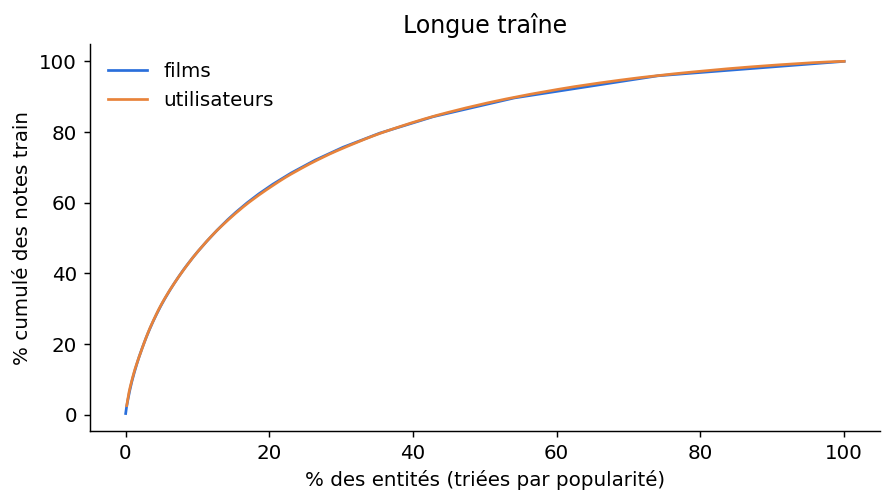
\includegraphics[width=0.55\linewidth]{eda/03_long_tail.png}
\caption{La \og longue traîne \fg : quelques films ont beaucoup de notes, une foule de
films en ont très peu. 21\,\% des notes de test portent sur un film qui a moins de
5 notes d'entraînement.}
\end{figure}

\subsection{La régularisation}\label{sec:reg}

La régularisation est le remède au surapprentissage. On ajoute une \textbf{pénalité}
qui dit à la méthode : \og reste prudente, ne t'éloigne de la valeur par défaut que si
les données le justifient vraiment \fg.

La force de cette pénalité est un bouton qu'on règle, souvent noté $\lambda$ (lambda) :
\begin{itemize}
  \item $\lambda$ trop petit : la méthode croit tout, elle surapprend ;
  \item $\lambda$ trop grand : la méthode ne croit rien, elle répond toujours la valeur par défaut ;
  \item le bon $\lambda$ : on essaie plusieurs valeurs et on garde la meilleure en validation.
\end{itemize}
Les réglages choisis à la main ($\lambda$, le rang, le nombre de voisins\dots) s'appellent
des \textbf{hyperparamètres}. Les nombres que la méthode apprend toute seule s'appellent
des \textbf{paramètres}.

%=============================================================================
\section{Vue d'ensemble des méthodes}
%=============================================================================

\begin{figure}[H]
\centering
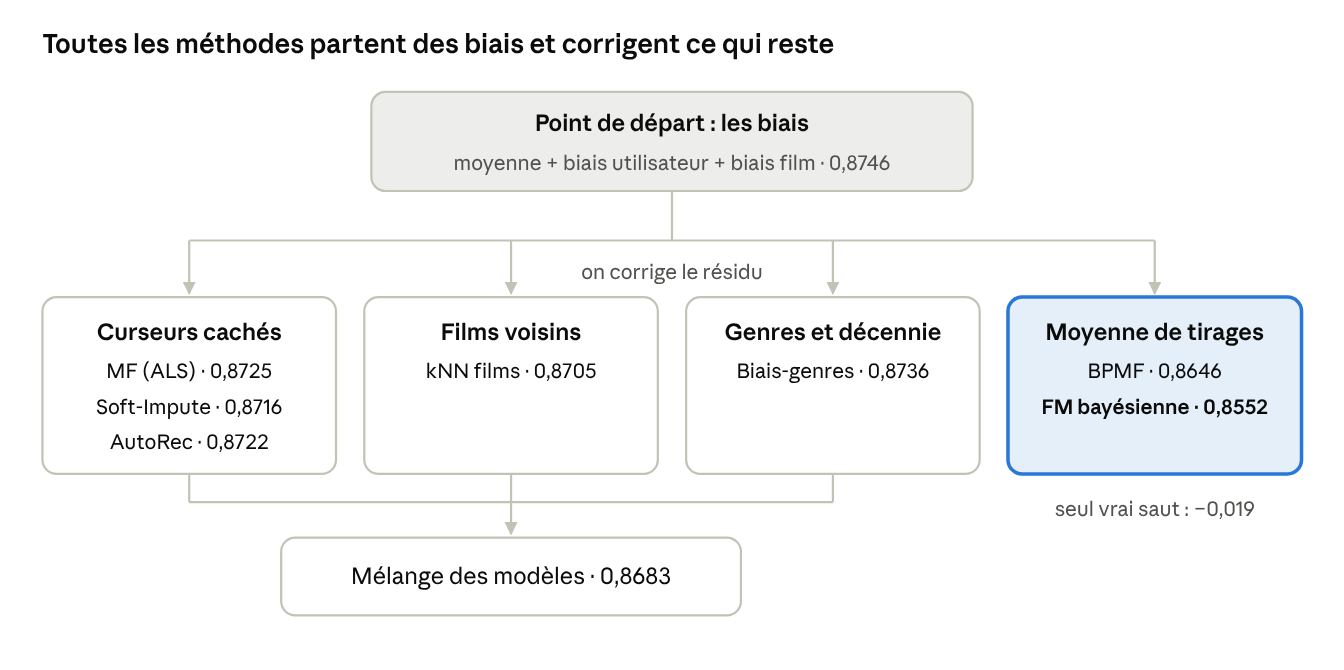
\includegraphics[width=\linewidth]{carte_methodes.png}
\caption{Toutes les méthodes partent des biais et corrigent ce qui reste. Les nombres
sont les RMSE sur le test (plus bas = mieux).}
\end{figure}

On part toujours d'une méthode très simple, les \textbf{biais}. Chaque autre méthode
ajoute sa propre correction : des curseurs cachés, des films voisins ou des genres.
L'approche bayésienne, encadrée, fait la moyenne de milliers de solutions au lieu d'en
choisir une, et c'est elle qui gagne.

%=============================================================================
\section{Méthode 1 --- La moyenne, puis les biais}\label{sec:biais}
%=============================================================================

\begin{enbref}
Chaque utilisateur a sa sévérité, chaque film sa réputation. Les additionner à la
moyenne suffit à faire passer l'erreur de 1,037 à \textbf{0,875}. C'est notre méthode
de référence (\emph{baseline}), celle qu'il faut battre.
\end{enbref}

\subsection{Étape 0 : la moyenne}

La prédiction la plus simple : répondre partout la note moyenne, environ 3,5.
Erreur : \textbf{1,037}.

\subsection{Étape 1 : ajouter les biais}

Un \emph{biais} est une tendance systématique. Il y en a deux :
\begin{itemize}
  \item \textbf{le biais de l'utilisateur} $b_u$ : Bob est sévère, il note en moyenne
        0,5 en dessous des autres ($b_u = -0{,}5$) ;
  \item \textbf{le biais du film} $b_i$ : Le Parrain est adulé, il reçoit en moyenne
        0,8 au-dessus ($b_i = +0{,}8$).
\end{itemize}
La prédiction devient une addition :
\[
  \rhat_{ui} = \mu + b_u + b_i .
\]

\begin{exemple}
Bob et Le Parrain : $3{,}5 - 0{,}5 + 0{,}8 = \mathbf{3{,}8}$ étoiles.
\end{exemple}

\subsection{Où intervient la régularisation}

Un film vu une seule fois, et noté 5 : son biais serait de $+1{,}5$. C'est sûrement
exagéré, une seule personne ne suffit pas. La régularisation tire le biais vers 0
quand le film a peu de notes. Concrètement :
\[
  b_i = \frac{\text{somme des écarts du film à la prédiction}}{\text{nombre de notes du film} + \lambda} .
\]
Avec $\lambda = 2$ : un film à 1 note voit son écart divisé par 3 au lieu de 1 (forte
prudence) ; un film à 200 notes, par 202 au lieu de 200 (quasiment rien ne change).

\subsection{Comment on les calcule}

On calcule les biais des films en supposant connus ceux des utilisateurs, puis l'inverse,
et on recommence une vingtaine de fois. Chaque calcul est une simple moyenne : le tout
prend 0,01 seconde. Le meilleur réglage en validation est $\lambda = 2$.

\begin{retenir}
Toutes les méthodes suivantes partent des biais et essaient de prédire \textbf{ce qui
reste} : l'écart entre la vraie note et la prédiction des biais. On l'appelle le
\textbf{résidu}. Le résidu, c'est le goût personnel : \og Alice aime la science-fiction
plus que les gens en général \fg.
\end{retenir}

%=============================================================================
\section{Méthode 2 --- La factorisation de matrice}\label{sec:mf}
%=============================================================================

\begin{enbref}
On décrit chaque utilisateur et chaque film par quelques \og curseurs \fg cachés,
inventés par la méthode, puis on mesure leur accord. C'est la méthode exigée par le
sujet. Gain faible chez nous : \textbf{0,8725} contre 0,8746, et seulement si la
régularisation est bien réglée.
\end{enbref}

\subsection{L'intuition}

Imaginons qu'on décrive chaque film par deux curseurs, \og action \fg et \og romance \fg,
et chaque utilisateur par deux curseurs, \og aime l'action \fg et \og aime la romance \fg.

\begin{center}
\begin{tabular}{lcc}
\toprule
 & action & romance \\
\midrule
Film : Alien & 0,9 & 0,1 \\
Utilisatrice : Alice & 0,8 & $-0{,}5$ \\
\bottomrule
\end{tabular}
\end{center}

Pour savoir si Alice aimera Alien, on multiplie curseur par curseur et on additionne.
Ce calcul s'appelle le \textbf{produit scalaire} :

\begin{exemple}
$0{,}9 \times 0{,}8 + 0{,}1 \times (-0{,}5) = 0{,}72 - 0{,}05 = \mathbf{+0{,}67}$.
Les goûts d'Alice collent au film : bonus de 0,67 étoile, ajouté aux biais.
\end{exemple}

La formule complète ajoute ce bonus aux biais :
\[
  \rhat_{ui} = \mu + b_u + b_i + p_u^\top q_i ,
\]
où $p_u$ est la liste des curseurs de l'utilisateur, $q_i$ celle du film, et
$p_u^\top q_i$ leur produit scalaire (le petit $\top$ est une convention d'écriture).

L'essentiel : \textbf{on ne choisit pas les curseurs}. La méthode les invente seule à
partir des notes. Ils sont cachés (on dit \emph{facteurs latents}) et souvent impossibles
à nommer. Leur nombre s'appelle le \textbf{rang} (chez nous, de 10 à 20).

Pourquoi \og factorisation \fg : le grand tableau $610 \times 4\,980$ est approché par
le produit de deux petits tableaux, $610 \times \text{rang}$ (les utilisateurs) et
$\text{rang} \times 4\,980$ (les films). Comme $12 = 3 \times 4$.

\subsection{Deux façons de trouver les curseurs}

On cherche les curseurs qui reproduisent au mieux les notes connues, avec une pénalité
pour ne pas surapprendre (deux boutons : $\lambda_f$ pour les curseurs, $\lambda_b$ pour
les biais).

\textbf{ALS (moindres carrés alternés).} Chercher les deux tableaux à la fois est
difficile. Mais si l'on fige les films, trouver les utilisateurs devient facile : c'est
une régression linéaire, qui se résout d'un coup par une formule. On alterne donc :
\begin{enumerate}
  \item on fige les films, on calcule les meilleurs utilisateurs ;
  \item on fige les utilisateurs, on calcule les meilleurs films ;
  \item on recommence (15 fois suffisent).
\end{enumerate}

\textbf{SGD (descente de gradient stochastique).} On prend les notes une par une. Pour
chacune, on regarde l'erreur, et on pousse un tout petit peu les curseurs de l'utilisateur
et du film dans la direction qui réduit cette erreur. On fait plusieurs passages sur toutes
les notes. La taille de chaque petit pas est un réglage de plus.

\begin{center}
\begin{tabular}{lll}
\toprule
 & \textbf{ALS} & \textbf{SGD} \\
\midrule
Principe & alterner deux problèmes faciles & petits pas, note par note \\
Réglages & $\lambda$, rang & $\lambda$, rang, taille du pas, nombre de passages \\
Stabilité & très stable & sensible à la taille du pas \\
RMSE test & \textbf{0,8725} & 0,8775 (pire que les biais) \\
\bottomrule
\end{tabular}
\end{center}

\textbf{ALS-WR} est une variante où la pénalité d'un utilisateur grandit avec son nombre
de notes. Chez nous, elle ne fait pas mieux que les biais (0,8746).

\subsection{Ce que nous avons appris}

\begin{figure}[H]
\centering
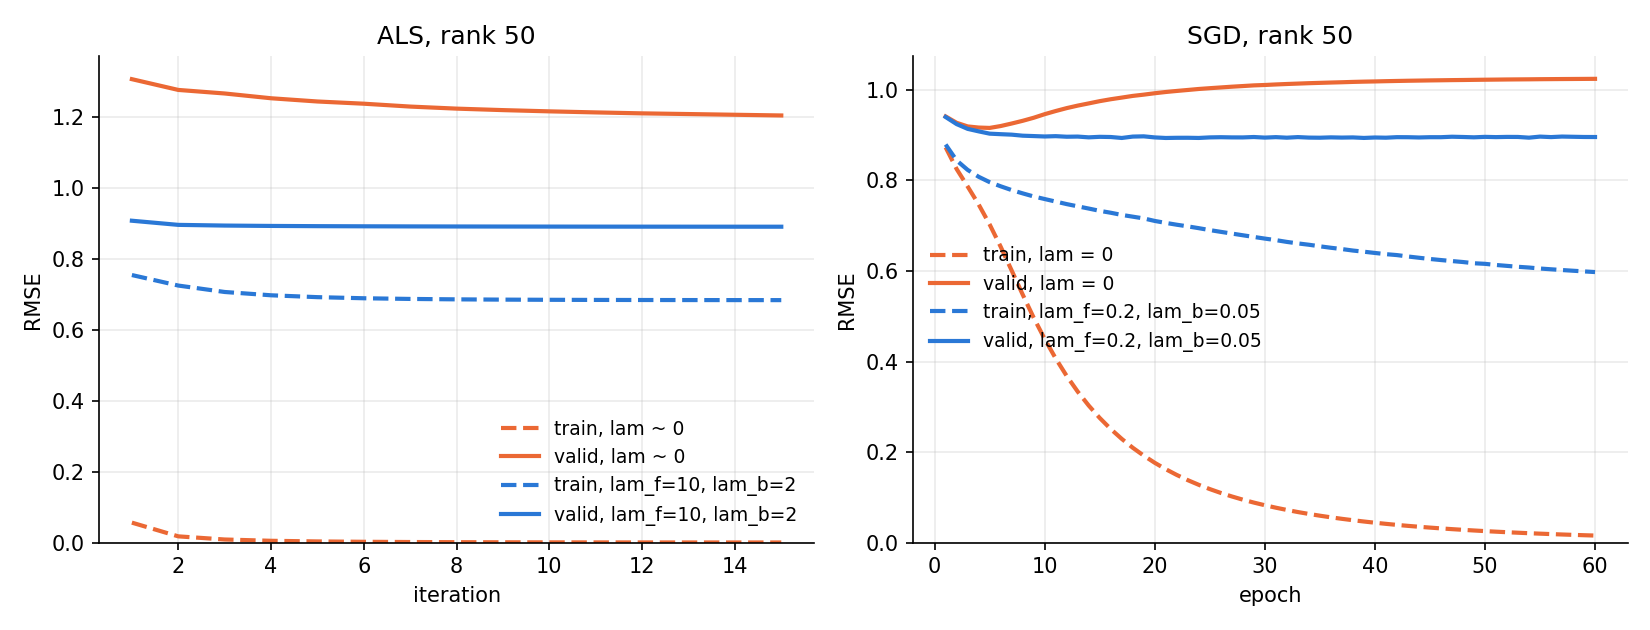
\includegraphics[width=0.85\linewidth]{mf_learning_curves.png}
\caption{Erreur au fil des itérations, sur l'entraînement et la validation, pour
plusieurs forces de pénalité.}
\end{figure}

Tout se joue sur la force de la pénalité $\lambda_f$ :
\begin{itemize}
  \item sans pénalité : erreur proche de 0 sur l'entraînement, plus de 1,0 en validation.
        C'est du surapprentissage pur ;
  \item pénalité de 15 ou plus : les curseurs sont écrasés à 0, on retombe exactement
        sur les biais ;
  \item la bonne zone est étroite, autour de 10. Une fois $\lambda_f$ bien choisi, le
        rang compte peu.
\end{itemize}
Le gain reste faible parce qu'avec 3 notes par film en médiane, il n'y a pas assez
d'information pour placer les curseurs de la plupart des films.

%=============================================================================
\section{Méthode 3 --- Soft-Impute}\label{sec:si}
%=============================================================================

\begin{enbref}
Même but que la factorisation, mais le nombre de curseurs n'est pas fixé à l'avance :
la méthode garde automatiquement ce qu'il faut. RMSE test : \textbf{0,8716}, en
4,7 secondes.
\end{enbref}

\subsection{L'idée : remplir, simplifier, recommencer}

On travaille sur les résidus (notes moins biais) et on répète une boucle :
\begin{enumerate}
  \item \textbf{remplir} : on met dans les cases vides notre meilleure devinette du moment
        (0 au départ) ; les cases connues gardent leur vraie valeur ;
  \item \textbf{simplifier} : on \og lisse \fg ce tableau complet pour n'en garder que
        les grandes tendances ;
  \item on recommence avec ce tableau lissé comme nouvelle devinette, jusqu'à ce que
        plus rien ne bouge.
\end{enumerate}

\subsection{Comment on simplifie : la SVD}

Tout tableau de nombres peut s'écrire comme une somme de \og motifs \fg, rangés du plus
important au plus faible. C'est la \textbf{SVD} (décomposition en valeurs singulières).
Chaque motif a une force, appelée \emph{valeur singulière}. On peut penser à un son
décomposé en notes de musique, des plus fortes aux plus faibles.

Soft-Impute retire la même quantité $\tau$ (tau) à la force de chaque motif :
\begin{itemize}
  \item un motif fort (force 50) devient 40 : il reste ;
  \item un motif faible (force 6) tombe à 0 : il disparaît.
\end{itemize}
Les motifs faibles sont surtout du bruit : on les supprime. C'est le sens de \emph{soft} :
on rabote tout, on ne coupe pas net. $\tau$ joue le rôle de $\lambda$ ; notre meilleur
réglage est $\tau = 10$. Avec $\tau \geq 20$, tous les motifs disparaissent et on retombe
sur les biais.

\begin{center}
\begin{tabular}{lll}
\toprule
 & \textbf{Factorisation (ALS)} & \textbf{Soft-Impute} \\
\midrule
Nombre de curseurs & fixé à l'avance (le rang) & choisi automatiquement par $\tau$ \\
Ce qu'on manipule & deux petits tableaux & le grand tableau complet \\
Réglages & rang et $\lambda$ & $\tau$ seulement \\
RMSE test & 0,8725 & 0,8716 \\
\bottomrule
\end{tabular}
\end{center}

%=============================================================================
\section{Méthode 4 --- Les plus proches voisins}\label{sec:knn}
%=============================================================================

\begin{enbref}
Pour deviner votre note sur un film, on regarde comment vous avez noté les films qui lui
ressemblent. RMSE test : \textbf{0,8705}, la meilleure des méthodes \og simples \fg.
\end{enbref}

\subsection{L'intuition}

\og Vous avez adoré Alien et Terminator, vous aimerez sûrement Predator. \fg
Aucun curseur caché : on compare directement les films entre eux. Le nom kNN vient de
l'anglais \emph{k nearest neighbours}, les $k$ plus proches voisins.

\subsection{Pas à pas, pour la note d'Alice sur Predator}

\begin{enumerate}
  \item \textbf{Mesurer la ressemblance entre films.} Deux films se ressemblent si les
        gens qui ont vu les deux réagissent pareil : ceux qui aiment l'un plus que prévu
        aiment aussi l'autre plus que prévu. On mesure cela par une \emph{corrélation},
        un nombre entre $-1$ (opposés) et $1$ (identiques).
  \item \textbf{Se méfier des petits échantillons.} Si deux films n'ont que 2 spectateurs
        en commun, leur ressemblance n'est pas fiable. On la multiplie par
        $\frac{n}{n + 100}$, où $n$ est le nombre de spectateurs communs : avec 5 spectateurs,
        elle est presque annulée ($5/105 \approx 0{,}05$) ; avec 500, elle est presque
        intacte ($500/600 \approx 0{,}83$).
  \item \textbf{Choisir les voisins.} Parmi les films qu'Alice a notés, on garde les
        $k = 40$ plus ressemblants à Predator.
  \item \textbf{Faire la moyenne.} On regarde l'écart entre la note d'Alice et ce que
        prévoyaient les biais, pour chaque voisin. On fait la moyenne de ces écarts,
        pondérée par la ressemblance, et on l'ajoute aux biais.
\end{enumerate}

\subsection{Notre correction : \texorpdfstring{$\beta$}{beta}}

La formule du cours a un défaut ici : si Alice n'a qu'un voisin, et très peu ressemblant,
la formule recopie quand même tout son écart. Avec 1\,\% de notes connues, ce cas est
fréquent. Nous ajoutons donc un petit nombre $\beta = 0{,}2$ au dénominateur de la moyenne.

\begin{exemple}
Deux voisins, de ressemblances 0,6 et 0,2, sur lesquels Alice a été $+1$ et $-1$ au-dessus
des biais. Moyenne pondérée sans $\beta$ :
$\frac{0{,}6 \times 1 + 0{,}2 \times (-1)}{0{,}6 + 0{,}2} = \frac{0{,}4}{0{,}8} = +0{,}5$.
Avec $\beta = 0{,}2$ : $\frac{0{,}4}{0{,}2 + 0{,}8} = +0{,}4$. La correction est plus prudente.
\end{exemple}

Effet mesuré en validation : 0,908 sans $\beta$, \textbf{0,885} avec.

\subsection{Où il aide}

Le kNN brille sur les films populaires (50 notes et plus) : erreur réduite de 0,016 par
rapport aux biais. Sur les films à 1 ou 2 notes, il fait un peu pire : pas assez de
spectateurs pour trouver des voisins fiables.

%=============================================================================
\section{Méthode 5 --- Les biais guidés par les genres}\label{sec:genres}
%=============================================================================

\begin{enbref}
On utilise une information en plus des notes : le genre et l'année de chaque film.
Gain global minuscule (0,8736 contre 0,8746), mais c'est la seule méthode \og simple \fg
qui aide sur les films presque jamais notés.
\end{enbref}

Avec les biais classiques, un film sans note a un biais de 0 : on lui prédit la moyenne.
Or on sait des choses sur lui. Un documentaire des années 1950 n'est pas noté comme une
comédie d'horreur récente. L'idée : au lieu de tirer le biais d'un film vers 0, on le
tire vers \textbf{ce que prédisent son genre, sa décennie et sa popularité}.
\begin{enumerate}
  \item On apprend combien chaque genre et chaque décennie rapporte en moyenne (par
        exemple, fictif : \og Film-Noir \fg $+0{,}3$, \og Horror \fg $-0{,}4$).
        C'est une régression linéaire.
  \item Pour chaque film, cette estimation devient le point de départ de son biais.
  \item Un film très noté s'éloigne de ce point de départ ; un film peu noté y reste.
\end{enumerate}
La popularité (le nombre de notes du film) aide aussi : les films rarement notés sont en
moyenne moins bien notés.

Sur les films à 1 ou 2 notes, c'est la seule de ces méthodes qui bat les biais (0,940
contre 0,944). Ces informations resservent, plus efficacement, dans la FM bayésienne.

%=============================================================================
\section{Méthode 6 --- Le mélange de méthodes}\label{sec:melange}
%=============================================================================

\begin{enbref}
On combine les prédictions de cinq méthodes. Le mélange fait mieux que chacune :
\textbf{0,8683} contre 0,8705 pour la meilleure seule.
\end{enbref}

C'est la sagesse des foules : si plusieurs experts se trompent \textbf{à des endroits
différents}, leur avis combiné est plus juste. Le kNN est fort sur les films populaires,
les biais-genres sur les films rares : en les combinant, on profite des deux.

\begin{enumerate}
  \item On entraîne les cinq méthodes (biais, biais-genres, Soft-Impute, kNN, ALS) sur
        90\,\% de l'entraînement.
  \item Chacune prédit les 10\,\% de validation.
  \item On cherche les poids qui combinent le mieux ces prédictions :
        \[ \rhat = w_0 + w_1 \rhat^{(1)} + w_2 \rhat^{(2)} + \dots + w_5 \rhat^{(5)} , \]
        où $\rhat^{(m)}$ est la prédiction de la méthode numéro $m$ et $w_m$ son poids.
        C'est une régression \emph{ridge} : une régression linéaire avec un peu de
        régularisation.
  \item On réentraîne les cinq méthodes sur tout l'entraînement et on applique ces poids.
\end{enumerate}

Pourquoi apprendre les poids sur la validation et pas sur l'entraînement ? Sur
l'entraînement, les méthodes qui surapprennent ont l'air excellentes ; le mélange leur
donnerait trop de poids.

\begin{center}
\begin{tabular}{lr}
\toprule
\textbf{Méthode} & \textbf{Poids appris} \\
\midrule
kNN & 0,94 \\
Biais-genres & 0,72 \\
ALS & 0,29 \\
Soft-Impute & 0,06 \\
Biais & $-1{,}01$ \\
\bottomrule
\end{tabular}
\end{center}

Le poids négatif des biais n'est pas absurde : toutes les méthodes contiennent déjà les
biais, on les retire une fois pour ne pas les compter plusieurs fois. Le mélange garde
donc surtout \textbf{les corrections} apportées par chaque méthode.

%=============================================================================
\section{Méthode 7 --- AutoRec, un réseau de neurones}\label{sec:autorec}
%=============================================================================

\begin{enbref}
Un petit réseau de neurones (\emph{deep learning}) apprend à compresser puis
reconstruire les notes d'un film. Sur nos données, il ne fait pas mieux que les méthodes
simples : \textbf{0,8722}, et il n'améliore pas le mélange.
\end{enbref}

\subsection{L'intuition : compresser puis décompresser}

Un \emph{auto-encodeur} est un réseau qui apprend à recopier son entrée en la faisant
passer par un goulot d'étranglement :
\begin{enumerate}
  \item \textbf{entrée} : la colonne d'un film, soit les notes des 610 utilisateurs
        (trouée : la plupart sont inconnues) ;
  \item \textbf{compression} : le réseau la résume en 500 nombres (la \emph{couche cachée}) ;
  \item \textbf{décompression} : à partir de ce résumé, il reconstruit les 610 notes,
        \textbf{y compris celles qui manquaient}.
\end{enumerate}
On l'entraîne à bien reconstruire les notes connues ; les notes inconnues sortent
\og gratuitement \fg de la reconstruction. Ce sont nos prédictions.

Les 500 nombres du résumé jouent le rôle des curseurs de la factorisation. La différence :
grâce à une fonction appelée \emph{sigmoïde}, le réseau peut apprendre des relations plus
complexes qu'une simple multiplication-addition (on dit \emph{non linéaires}).

\subsection{Ce que nous avons testé}

\begin{center}
\begin{tabular}{lc}
\toprule
\textbf{Variante} & \textbf{RMSE test} \\
\midrule
Par film, sur les notes brutes & 0,912 (pire que les biais) \\
Par utilisateur, sur les résidus & 0,883 \\
\textbf{Par film, sur les résidus} & \textbf{0,8722} \\
Par film, résidus, variante \og Sparse FC \fg & 0,873 \\
\bottomrule
\end{tabular}
\end{center}

Le réseau marche beaucoup mieux sur les résidus que sur les notes brutes : les biais
font le gros du travail, le réseau n'a plus qu'à apprendre les goûts.

\subsection{Pourquoi le deep learning échoue ici}

Le réseau a des centaines de milliers de paramètres pour seulement 31\,600 notes. Il
surapprend très vite, même avec une forte régularisation et en arrêtant l'entraînement
au meilleur moment. C'est cohérent avec la littérature : sur des données aussi creuses,
les méthodes bayésiennes font mieux que le deep learning.

%=============================================================================
\section{Méthode 8 --- Les méthodes bayésiennes}\label{sec:bayes}
%=============================================================================

\begin{enbref}
Au lieu de chercher \emph{la} meilleure solution, on tire au sort des milliers de
solutions plausibles et on fait la moyenne de leurs prédictions. C'est notre meilleur
résultat et le seul vrai saut : la FM bayésienne atteint \textbf{0,8552}, soit 0,019 de
mieux que les biais, en 60 secondes.
\end{enbref}

\subsection{L'idée : faire la moyenne au lieu de choisir}

Toutes les méthodes précédentes cherchent une seule solution, les \og meilleurs \fg
curseurs. Mais avec si peu de notes, beaucoup de solutions différentes expliquent les
données presque aussi bien. En choisir une, c'est parier.

L'approche bayésienne ne parie pas. Elle part d'une supposition raisonnable (l'\emph{a
priori} : \og les curseurs sont probablement petits \fg), la corrige avec les données,
puis tire au sort des milliers de solutions compatibles avec les deux. La prédiction
finale est la \textbf{moyenne} de leurs prédictions :
\[
  \rhat_{ui} = \frac{1}{S} \sum_{s=1}^{S} \rhat^{(s)}_{ui} ,
\]
où $\rhat^{(s)}_{ui}$ est la prédiction du tirage numéro $s$ et $S$ le nombre de tirages.

\subsection{Comment on tire ces solutions : l'échantillonnage de Gibbs}

C'est la même alternance que l'ALS, avec du hasard :
\begin{enumerate}
  \item on fige les films et on \textbf{tire au sort} des curseurs utilisateurs plausibles,
        au lieu de prendre les meilleurs ;
  \item on fige les utilisateurs et on tire des curseurs films plausibles ;
  \item on tire aussi la force de la régularisation ;
  \item on note la prédiction obtenue, et on recommence des centaines de fois.
\end{enumerate}
Les premiers tirages, encore mauvais, sont jetés (le \emph{burn-in}).

\begin{figure}[H]
\centering
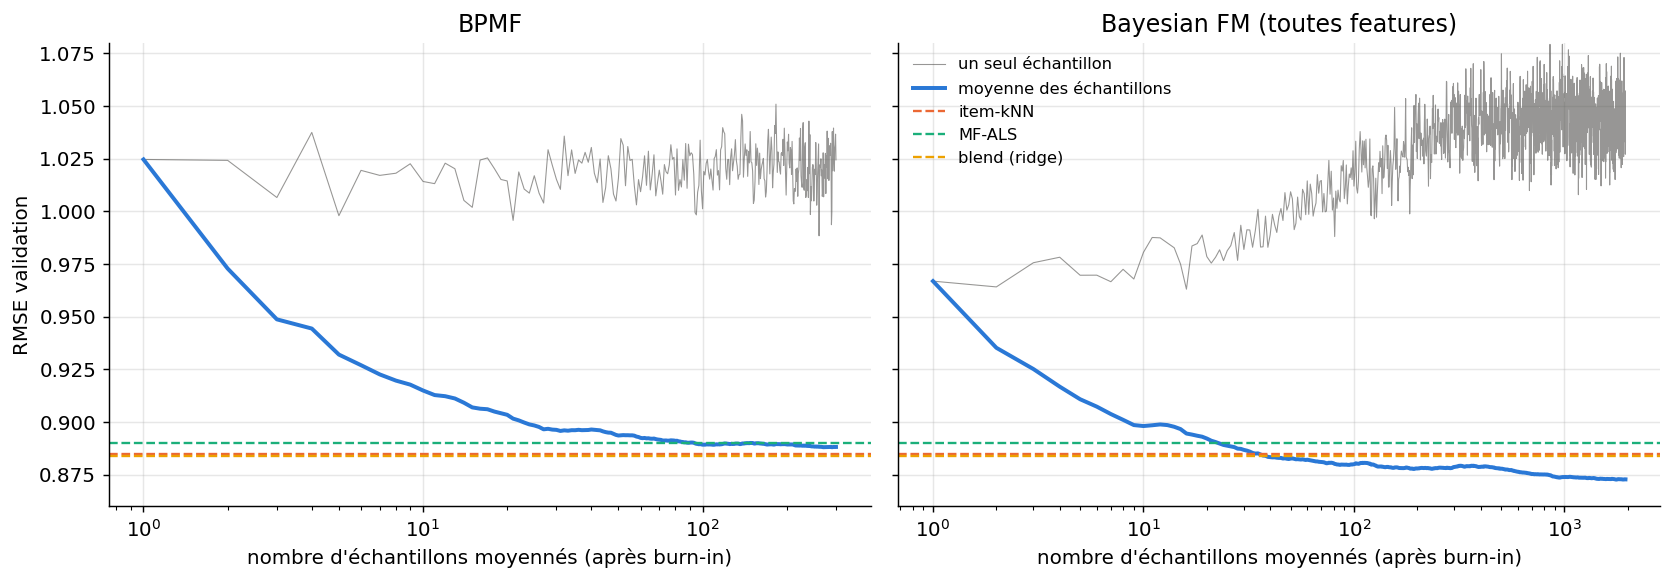
\includegraphics[width=0.7\linewidth]{bayes/rmse_vs_samples.png}
\caption{Erreur d'un tirage seul et de la moyenne des tirages, en fonction du nombre de
tirages.}
\end{figure}

Fait frappant : un tirage seul est mauvais (erreur d'environ 1,03, pire que la moyenne
globale). La moyenne de 2\,000 tirages descend à 0,873 en validation. Tout le gain vient
de la moyenne.

Autre avantage : plus de $\lambda$ à régler à la main. La force de la régularisation est
elle-même tirée au sort et apprise des données.

\subsection{BPMF : la factorisation bayésienne}

BPMF (\emph{Bayesian Probabilistic Matrix Factorization}) est exactement la factorisation
de la section~\ref{sec:mf}, biais compris, en version bayésienne. Résultat :
\textbf{0,8646} (rang 20, 300 tirages, 44 secondes).

\subsection{FM bayésienne : on ajoute des informations}

Une \emph{machine de factorisation} (FM) est une factorisation généralisée : elle peut
recevoir d'autres informations que \og qui \fg et \og quel film \fg, chacune avec ses
propres curseurs. Nous lui en donnons trois :
\begin{itemize}
  \item \textbf{les films notés par l'utilisateur} : avoir vu tel film dit quelque chose
        de vos goûts, quelle que soit la note (c'est l'idée de la méthode \emph{SVD++}) ;
  \item \textbf{les utilisateurs qui ont noté le film} : la même idée côté film, le public
        d'un film décrit le film ;
  \item \textbf{les genres et la décennie} du film.
\end{itemize}
Nous utilisons la bibliothèque \texttt{myfm}, qui fait l'échantillonnage de Gibbs pour nous.

\subsection{Quelle information compte le plus ? L'ablation}

Une \emph{ablation} consiste à ajouter (ou retirer) une information à la fois pour mesurer
son apport.

\begin{figure}[H]
\centering
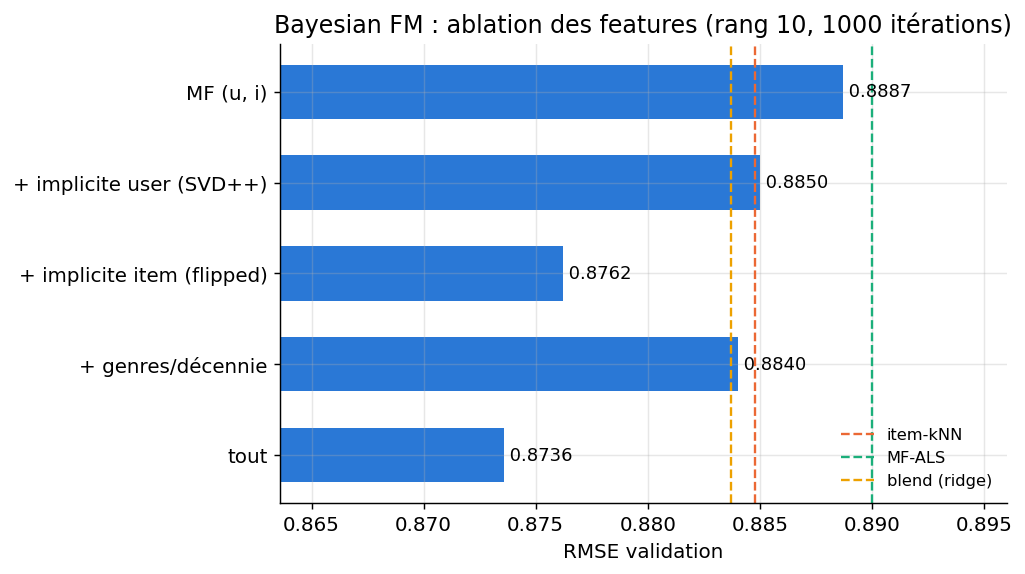
\includegraphics[width=0.7\linewidth]{bayes/ablation.png}
\caption{Erreur de validation de la FM bayésienne selon les informations ajoutées
(1\,000 tirages). \og implicite user \fg = films notés par l'utilisateur ;
\og implicite item \fg = utilisateurs qui ont noté le film ; les lignes verticales
rappellent le kNN, l'ALS et le mélange.}
\end{figure}

\begin{center}
\begin{tabular}{lc}
\toprule
\textbf{Configuration} & \textbf{RMSE validation} \\
\midrule
FM de base (= factorisation bayésienne) & 0,8887 \\
+ films notés par l'utilisateur & 0,8850 \\
+ genres et décennie & 0,8840 \\
+ \textbf{utilisateurs qui ont noté le film} & \textbf{0,8762} \\
Les trois ensemble (2\,000 tirages au lieu de 1\,000) & \textbf{0,8728} \\
\bottomrule
\end{tabular}
\end{center}

Le plus utile, de loin : savoir \textbf{qui a regardé le film}, plus que les notes
elles-mêmes. Pour un film à 3 notes, ces 3 spectateurs en disent beaucoup sur le type de
film. Sur les données de la plateforme (entraînement + test), la FM bayésienne tourne en
93 secondes, loin de la limite de 1\,200.

%=============================================================================
\section{Comparatif et leçons}
%=============================================================================

\begin{center}
\small
\begin{tabularx}{\linewidth}{@{}lXlrr@{}}
\toprule
\textbf{Méthode} & \textbf{Idée en une phrase} & \textbf{Réglage clé} & \textbf{RMSE} & \textbf{Temps} \\
\midrule
\textbf{FM bayésienne} & moyenne de milliers de factorisations + qui a vu quoi + genres & appris seul & \textbf{0,8552} & 60 s \\
BPMF & moyenne de milliers de factorisations & appris seul & 0,8646 & 44 s \\
Mélange & combinaison pondérée de 5 méthodes & ridge & 0,8683 & 7,7 s \\
kNN films & écarts sur les films ressemblants & $k$, shrink, $\beta$ & 0,8705 & 1,1 s \\
Soft-Impute & remplir, lisser par SVD, recommencer & $\tau$ & 0,8716 & 4,7 s \\
AutoRec & réseau qui compresse puis reconstruit & $\lambda$, arrêt & 0,8722 & 17 s \\
MF -- ALS & curseurs cachés, calcul alterné & $\lambda_f$, $\lambda_b$ & 0,8725 & 1,5 s \\
Biais + genres & biais tiré vers ce que prédit le genre & $\lambda$ & 0,8736 & 0,04 s \\
\textbf{Biais} (référence) & moyenne + sévérité + réputation & $\lambda$ & \textbf{0,8746} & 0,01 s \\
MF -- ALS-WR & ALS, pénalité selon le nombre de notes & $\lambda$ & 0,8746 & 1,5 s \\
MF -- SGD & curseurs cachés, petits pas & $\lambda$, pas & 0,8775 & 0,5 s \\
Moyenne globale & la même note partout & aucun & 1,0369 & 0 s \\
\bottomrule
\end{tabularx}
\end{center}

\subsection{Trois oppositions pour s'y retrouver}

\begin{itemize}
  \item \textbf{Curseurs cachés ou comparaison directe.} Factorisation, Soft-Impute,
        AutoRec et méthodes bayésiennes inventent des curseurs cachés. Le kNN compare
        directement les films entre eux.
  \item \textbf{Une solution ou une moyenne.} Toutes les méthodes choisissent une
        solution, sauf BPMF et la FM bayésienne qui en moyennent des milliers.
        C'est ce qui fait la différence ici.
  \item \textbf{Notes seules ou informations en plus.} Biais-genres et FM bayésienne
        utilisent aussi les genres et l'année ; la FM utilise en plus \og qui a vu quoi \fg.
\end{itemize}

\subsection{Où chaque méthode aide}

\begin{figure}[H]
\centering
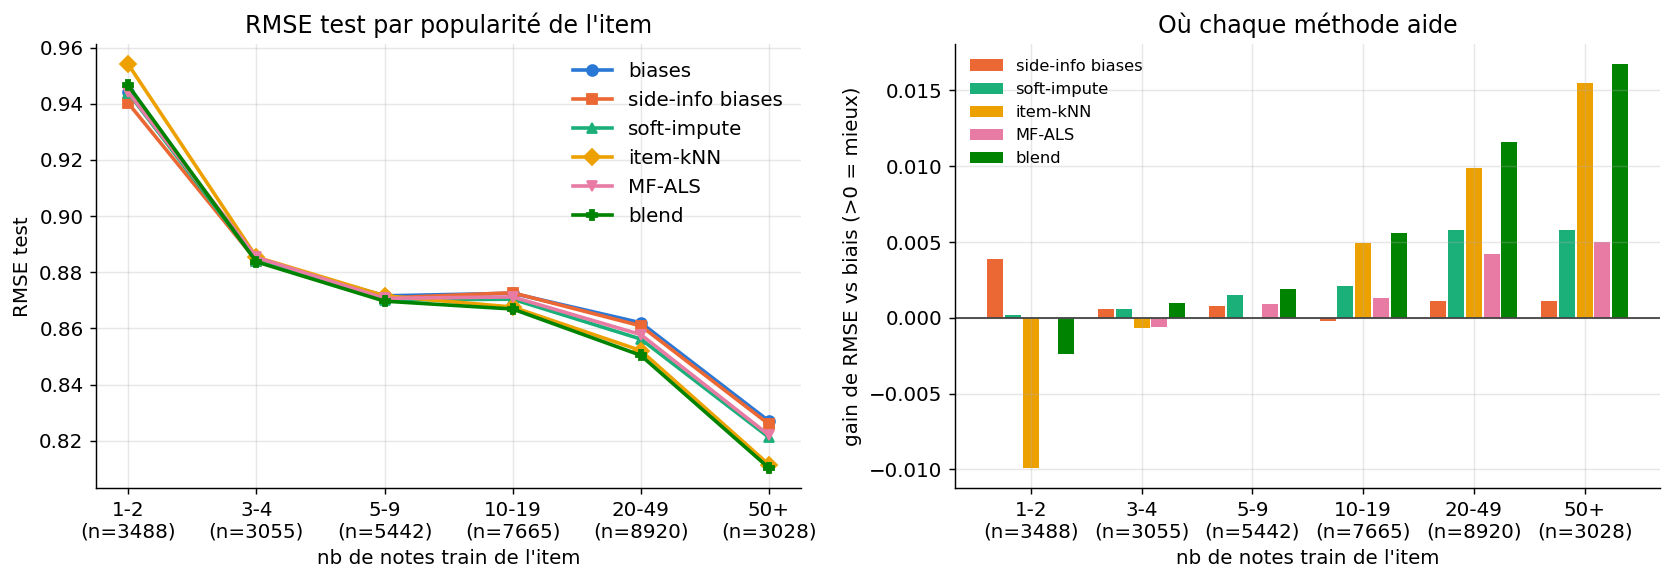
\includegraphics[width=0.9\linewidth]{alt/rmse_by_popularity.png}
\caption{Erreur de chaque méthode selon le nombre de notes du film.}
\end{figure}

Les films sont rangés en groupes selon leur nombre de notes (1--2, 3--4, \dots, 50 et plus).
Le kNN et Soft-Impute gagnent sur les films populaires ; seuls les biais-genres aident sur
les films à 1--2 notes.

\begin{retenir}
\begin{enumerate}[leftmargin=*]
  \item Avec 1\,\% de notes connues, les biais font 90\,\% du gain.
  \item Pour les méthodes à solution unique, le réglage de la régularisation compte plus
        que le choix de la méthode.
  \item Arrondir les prédictions à la demi-étoile ne change pas l'accuracy mais dégrade
        la RMSE de 0,012 : on n'arrondit pas.
  \item Sur des données aussi creuses, les méthodes bayésiennes font mieux que le deep
        learning.
\end{enumerate}
\end{retenir}

%=============================================================================
\section{Lire les formules des slides}
%=============================================================================

Cette section reprend, slide par slide, chaque formule et la traduit en français.

\subsection{Slide \og Les données \fg}

\begin{itemize}
  \item \textbf{Longue traîne} (figure de gauche) : voir la section~\ref{sec:reg}.
  \item \textbf{Spectre} (figure de droite) : les forces des motifs de la SVD
        (section~\ref{sec:si}), de la plus forte à la plus faible.
  \item \textbf{Bruit permuté} : on mélange les résidus au hasard pour détruire toute
        structure, puis on recalcule le spectre. Si le vrai spectre ressemble à celui du
        bruit, les motifs correspondants ne contiennent rien d'exploitable. Chez nous,
        c'est le cas au-delà d'environ 5 motifs : il reste très peu à apprendre après les biais.
\end{itemize}

\subsection{Slide \og Méthodes comparées \fg, ligne par ligne}

\textbf{Biais.} $\rhat_{ui} = \mu + b_u + b_i$, pénalité
$\lambda\bigl(\|b_u\|^2 + \|b_i\|^2\bigr)$.
La notation $\|b\|^2$ (\og norme au carré \fg) est la somme des carrés des nombres :
pour $b = (0{,}5 \,;\, -1)$, $\|b\|^2 = 0{,}25 + 1 = 1{,}25$. Elle mesure la \og taille \fg
des biais ; la pénaliser empêche les biais trop grands.

\textbf{Factorisation.} $\rhat_{ui} = \mu + b_u + b_i + p_u^\top q_i$ : le produit
scalaire de la section~\ref{sec:mf}. $\lambda_b$ et $\lambda_f$ sont deux boutons
distincts, pour les biais et pour les curseurs.

\textbf{ALS.} $p_u = (Q_u^\top Q_u + \lambda_f I)^{-1} Q_u^\top \tilde r_u$.
C'est la formule qui donne d'un coup les meilleurs curseurs de l'utilisateur $u$ quand
les films sont figés :
\begin{itemize}
  \item $Q_u$ : le tableau des curseurs des films que $u$ a notés ;
  \item $\tilde r_u$ : ses résidus sur ces films (le tilde signale \og note moins biais \fg) ;
  \item $I$ : la matrice identité, l'équivalent du nombre 1 pour les matrices ;
  \item $(\dots)^{-1}$ : l'inverse, l'équivalent de \og diviser par \fg pour les matrices.
\end{itemize}
Avec un seul curseur, elle devient une simple division :
$p = \dfrac{\sum q \times \tilde r}{\sum q^2 + \lambda_f}$. On reconnaît la formule des
biais : $\lambda_f$ au dénominateur rend le résultat prudent.

\textbf{Soft-Impute.} $\min_Z \tfrac12 \sum_{\text{obs.}} (r_{ui} - z_{ui})^2 + \tau \|Z\|_*$.
\begin{itemize}
  \item $\min_Z$ : chercher le tableau $Z$ qui rend l'expression la plus petite possible ;
  \item le premier terme oblige $Z$ à coller aux notes observées ;
  \item $\|Z\|_*$ (\og norme nucléaire \fg) : la somme des forces des motifs de $Z$. La
        pénaliser pousse $Z$ à n'avoir que peu de motifs ;
  \item \og seuillage des valeurs singulières \fg : retirer $\tau$ à chaque force et mettre
        à 0 celles qui deviennent négatives.
\end{itemize}

\textbf{kNN.} $\rhat_{ui} = \text{biais} + \dfrac{\sum_{j \in N_k(i;u)} s_{ij}\, e_{uj}}{\beta + \sum_j |s_{ij}|}$.
\begin{itemize}
  \item $N_k(i;u)$ : les $k$ films notés par $u$ qui ressemblent le plus à $i$ ;
  \item $s_{ij}$ : la ressemblance entre les films $i$ et $j$ ; $|s_{ij}|$ : sa valeur
        sans le signe ;
  \item $e_{uj}$ : le résidu de $u$ sur le voisin $j$ ;
  \item la fraction est la moyenne pondérée de l'exemple de la section~\ref{sec:knn} ;
  \item \og Pearson rétréci \fg $s_{ij} \frac{n_{ij}}{n_{ij} + 100}$ : la corrélation
        multipliée par le facteur de prudence, $n_{ij}$ étant le nombre de spectateurs communs.
\end{itemize}

\textbf{Biais + genres.} $b_i$ tiré vers $f_i^\top w$ : $f_i$ vaut 1 pour chaque genre
ou décennie du film et 0 sinon ; $w$ est ce que rapporte chaque genre ou décennie ; leur
produit scalaire est la somme des valeurs des genres du film.

\textbf{Mélange.} $\rhat_{ui} = w_0 + \sum_m w_m \rhat^{(m)}_{ui}$ : la combinaison
pondérée de la section~\ref{sec:melange}.

\textbf{AutoRec.} $\hat{e}_{\cdot i} = V\,\sigma(W e_{\cdot i} + b) + c$.
\begin{itemize}
  \item $e_{\cdot i}$ : la colonne des résidus du film $i$ (le point veut dire \og tous les
        utilisateurs \fg) ;
  \item $W$, $b$ : les paramètres de la compression ; $V$, $c$ : ceux de la décompression ;
  \item $\sigma$ (\og sigmoïde \fg) : une fonction qui écrase tout nombre entre 0 et 1
        ($\sigma(0) = 0{,}5$, $\sigma(5) \approx 0{,}99$, $\sigma(-5) \approx 0{,}01$) ;
  \item \og perte sur les notes observées \fg : l'erreur n'est mesurée que sur les cases connues.
\end{itemize}

\textbf{MF bayésienne.} \og A priori \fg, échantillonnage de Gibbs et
$\rhat_{ui} = \frac1S \sum_s \rhat^{(s)}_{ui}$ : voir la section~\ref{sec:bayes}.
\og SVD++ \fg désigne l'ajout des films notés par l'utilisateur.

\subsection{Les slides de résultats}

\begin{itemize}
  \item \textbf{Courbes d'apprentissage} (slide sur la régularisation) : l'erreur au fil
        des itérations. Une courbe d'entraînement qui descend pendant que celle de
        validation remonte, c'est du surapprentissage.
  \item \textbf{Ablation} (slide sur la MF bayésienne) : le tableau de la
        section~\ref{sec:bayes}.
  \item \textbf{Colonne \og s \fg} du tableau de résultats : le temps d'entraînement en secondes.
  \item \textbf{$-0{,}019$} : la baisse d'erreur de la FM bayésienne par rapport aux biais
        ($0{,}8746 \to 0{,}8552$).
\end{itemize}

%=============================================================================
\section{Où trouver quoi, et la suite}
%=============================================================================

\subsection{Le dépôt}

\begin{center}
\small
\begin{tabularx}{\linewidth}{@{}lX@{}}
\toprule
\textbf{Dossier ou fichier} & \textbf{Contenu} \\
\midrule
\texttt{generate.py} & le script noté par la plateforme (aujourd'hui : les biais) \\
\texttt{src/data.py} & chargement des données, découpage, RMSE et accuracy \\
\texttt{src/baselines.py} & moyenne et biais \\
\texttt{src/mf.py} & factorisation : ALS, ALS-WR, SGD \\
\texttt{src/soft\_impute.py} & Soft-Impute \\
\texttt{src/knn.py} & plus proches voisins \\
\texttt{src/side\_info.py} & biais guidés par les genres \\
\texttt{src/blend.py} & mélange \\
\texttt{src/autorec.py} & AutoRec \\
\texttt{src/bpmf.py}, \texttt{src/bfm.py} & BPMF et FM bayésienne \\
\texttt{experiments/} & les scripts qui lancent les expériences \\
\texttt{results/}, \texttt{figures/} & les chiffres et les graphiques produits \\
\texttt{docs/} & procédure, état de l'art, ce cours \\
\texttt{slides.pdf} & les slides du 15 octobre \\
\bottomrule
\end{tabularx}
\end{center}

\subsection{La suite}

\begin{enumerate}
  \item Mettre la FM bayésienne dans \texttt{generate.py}, pour obtenir un score officiel
        sur la plateforme.
  \item Essayer un mélange FM bayésienne + kNN + BPMF.
  \item Vérifier que les réglages tiennent sur entraînement + test (deux fois plus de notes).
  \item Fusionner la branche de travail dans \texttt{main} : c'est elle que la plateforme
        et les correcteurs regardent.
\end{enumerate}

%=============================================================================
\section{Glossaire}
%=============================================================================

\begin{center}
\small
\begin{tabularx}{\linewidth}{@{}lX@{}}
\toprule
\textbf{Mot} & \textbf{Sens simple} \\
\midrule
A priori & ce qu'on suppose avant de voir les données, corrigé ensuite par elles \\
Ablation & ajouter ou retirer un ingrédient à la fois pour mesurer son apport \\
Accuracy & pourcentage de notes devinées exactement, après arrondi à la demi-étoile \\
ALS & calcul alterné : on fige les films pour trouver les utilisateurs, puis l'inverse \\
Auto-encodeur & réseau qui compresse son entrée puis la reconstruit \\
Baseline & méthode simple de référence, à battre (chez nous : les biais) \\
Biais & tendance systématique : utilisateur sévère, film adulé \\
Burn-in & premiers tirages jetés, le temps que l'échantillonnage se stabilise \\
Corrélation & nombre entre $-1$ et $1$ qui mesure si deux séries varient ensemble \\
Facteurs latents & curseurs cachés inventés par la méthode pour décrire goûts et films \\
Filtrage collaboratif & deviner vos goûts à partir des notes des autres \\
Gibbs (échantillonnage) & tirer au sort une partie des inconnues en figeant les autres, en boucle \\
Hyperparamètre & réglage choisi à la main ($\lambda$, rang, $k$\dots), pas appris \\
kNN & $k$ plus proches voisins : s'appuyer sur les éléments les plus ressemblants \\
$\lambda$ (lambda) & force de la régularisation \\
Matrice & tableau de nombres \\
Norme & la \og taille \fg d'un vecteur ou d'une matrice \\
Norme nucléaire & somme des forces des motifs (valeurs singulières) d'un tableau \\
Paramètre & nombre appris par la méthode elle-même \\
Produit scalaire & multiplier deux vecteurs élément par élément, puis additionner \\
Rang & nombre de curseurs cachés par utilisateur et par film \\
Régression linéaire & trouver les poids qui expliquent au mieux une valeur par une somme pondérée \\
Régularisation & pénalité qui rend la méthode prudente, contre le surapprentissage \\
Résidu & ce que les biais n'expliquent pas : vraie note moins prédiction des biais \\
Ridge & régression linéaire avec régularisation \\
RMSE & erreur moyenne en étoiles, qui punit fort les grosses erreurs ; plus bas = mieux \\
SGD & descente de gradient : corriger les paramètres par petits pas, note par note \\
Sigmoïde ($\sigma$) & fonction qui écrase tout nombre entre 0 et 1 \\
Surapprentissage & apprendre l'entraînement par c\oe ur et mal deviner les notes nouvelles \\
SVD & décomposition d'un tableau en motifs, du plus fort au plus faible \\
Train / validation / test & le cours / l'examen blanc / le vrai examen \\
Valeur singulière & la force d'un motif de la SVD \\
Vecteur & liste de nombres \\
\bottomrule
\end{tabularx}
\end{center}

\end{document}
